\documentclass{article}
\usepackage[utf8]{inputenc}
\usepackage{authblk}
\usepackage{setspace}
\usepackage[margin=1.25in]{geometry}
\usepackage{graphicx}
\usepackage{xcolor}
\usepackage{float}
\graphicspath{ {./figures/} }
\usepackage{amsmath,amssymb,amsfonts}
\usepackage{booktabs}
\usepackage{natbib}
\usepackage{hyperref}
\hypersetup{colorlinks=true, linkcolor=blue, citecolor=blue, urlcolor=blue}

\title{\textbf{Fear Spikes and Next-Week Returns: Does an Elevated VIX Predict Higher US Equity Returns?}}
\author[1]{SIQuant Research}
\affil[1]{Hypothesis $\times$ Quant}
\date{\today}
\onehalfspacing

\begin{document}
\maketitle

\begin{abstract}
\noindent \textbf{Hypothesis:} $H_0$: the 60-day VIX z-score has no predictive power for the S\&P 500 return over the next five sessions; $H_1$: the slope is positive \\
\textbf{Data:} 2,450 daily observations, 2017-01-19 to 2026-10-16; 184 sessions with $z>2$ \\
\textbf{Method:} OLS with Newey--West HAC errors (10 lags) and a 2,000-draw circular-shift placebo; the decision needs both one-sided $p<0.05$ \\
\textbf{Results:} $\beta=-0.00023$ (HAC $t=-0.22$, $p=0.5858$; placebo $p=0.6067$), $R^2=0.0001$; mean next-week return 0.10\% after $z>2$ versus 0.26\% otherwise. \\
\textbf{Research decision:} \colorbox[rgb]{0.75,0.15,0.15}{\textcolor{white}{\textbf{\,REJECTED\,}}}
\end{abstract}

\section{Design}
The VIX z-score is computed from the 60 closes ending on day $t$ and the outcome is the log return from the close of $t$ to the close of $t+5$, so predictor and outcome do not overlap \citep{whaley2000investor}. The five-day overlap between neighbouring outcomes is handled with HAC errors (10 lags) and a circular-shift placebo.

\section{Results}
\begin{figure}[H]
\centering
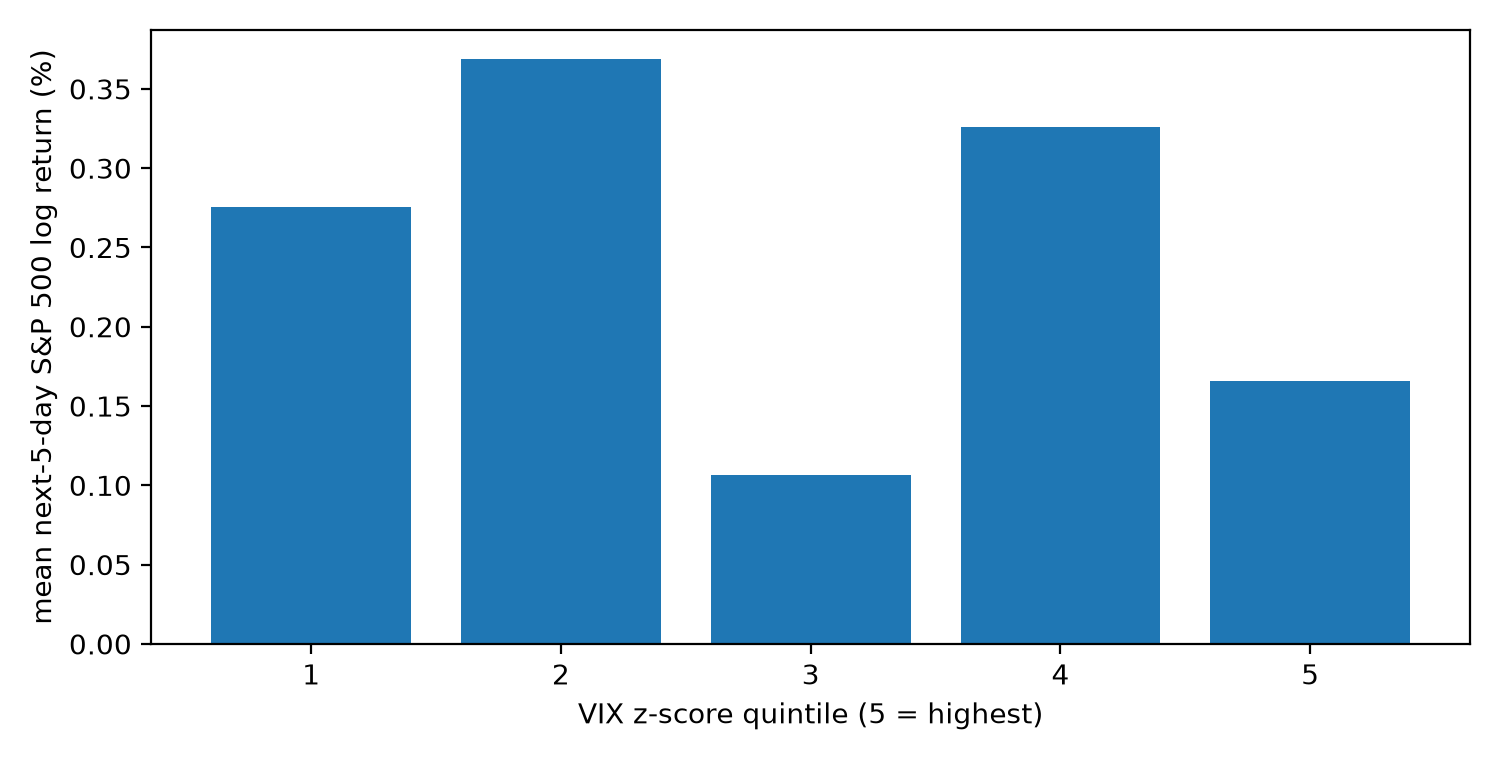
\includegraphics[width=0.8\textwidth]{fig1_vix_z_quintile_forward_return.png}
\caption{Mean next-week S\&P 500 return by quintile of the VIX z-score.}
\end{figure}

\section{Limitations}
The sample contains few independent volatility spikes (2018, 2020, 2022, 2025), so the effective sample is small. No transaction costs or timing frictions are modelled and the result is not a trading rule.


\bibliographystyle{plainnat}
\bibliography{references}

\end{document}
